\section{Systemtheoretische Vorbetrachtungen}
\subsection{Modellierung und Quadcoptersystem}
\subsubsection{Allgemeine Anforderungen an ein Dynamikmodell}
Unter einem Modell versteht man in der Philosophie eine Abbildung oder Repräsentation eines Objektes, eines Verhaltens oder eines Systems, das man verstehen möchte \ref{link:Modelle}.\\
Im Falle des Quadcopters galt es ein Dynamikmodell zu finden welches dessen Verhalten ausreichend gut abbildet um alle gesetzten Ziele zu erreichen. Aus dem primär, gesetzten Ziel, der Entwicklung eines flugfähigen Quadcopters, lassen sich Anforderungen ableiten.
Zum einen sollen die Vorhersagen des Modells über den tatsächlichen Zustand des Quadcopters nur bis auf einen maximalen Fehler abweichen von demjenigen Zustand, den man beobachten würde bei einem Quadcopter mit gleichen Input- und Systemparametern. Weicht auch nur ein vorhergesagter Wert weiter von seinem Soll ab als gewünscht ist das Modell unbrauchbar. Bei jedem Modell ist zu erwarten, dass die Vorhersagen in einer dynamischen Umwelt degradieren. Aus diesem Grund sollte die Qualität eines Modells auch abhängig von der Zeit betrachtet werden. Da für die Entwicklung eines Fluglagereglers nur Zustände innerhalb eines Flugintervalls vorhergesagt werden müssen, wurde von dem Modell nur erwartet, dass es über den Zeitraum von circa 5 Minuten vorhersagen innerhalb der Fehlerschranken liefert.\\
Wird ein Modell nicht Grund auf neu entwickelt, sondern aus einer Quelle herangezogen gilt es zu Validieren, dass das Modell den Anforderungen entspricht.\\
Das Flugdynamikmodell sowie die Implementierung eines Quadcopterreglerns wurden aus einem öffentlichen Repository bezogen und angepasst.
\begin{align}
	\label{simcon:simcon}\text{https://github.com/bobzwik/Quadcopter\_SimCon}
\end{align}
Da die Praktikabilität bei dieser Arbeit im Vordergrund steht wurde das Modell nach minimalen Plausibilitätstest für gut befunden und übernommen. Unter anderen Umständen ist es sinnvoll umfangreichere Tests an unbekannten Modellen oder Black-Box-Software durchzuführen.
Diese Tests könnten Mängel der Vorhersagegenauigkeit des Modells, invalide gewählte Inputparameter oder numerische Stabilitäts- und Konvergenzprobleme mit höherer Wahrscheinlichkeit zu Tage treffen lassen. Insgesammt stand der Nutzen für den Prototypen in keinem Verhältnis zu den Kosten sodass sich fokusiert wurde auf die korrekte Implementierung aller Schnittstellen. 
\subsubsection{Teilsysteme des Quadcopters}
Ein technisches System kann zur Veranschaulichung nahezu beliebig oft unterteilt werden. Naheliegend ist beispielsweise Hardware- und Softwarekomponenten zu trennen. In dieser Arbeit wurde ein anderer Ansatz verwendet. Geclustert wurden Teilsysteme nach ihren primär abgeleiteten Flussgrößen. Primärziel eines Motors ist beispielsweise einen Impulsfluss zu generieren und abzugeben. Aus diesem Grund wird er zum Impulsflusssystem zugeordnet und nicht zum Energieflusssystem. Mikrocontroller nehmen in der Funktion als Quadcopterregler Informationssignale, Energiesignale und technisch gesehen auch Impulse auf, geben aber primär Informationssignale ab.\\
Entsprechend wurde eine Klassifizierung zentraler Teilsysteme erstellt. Die Simulationssoftware umfasst nicht die Reglersoftware auf einem Mikrocontroller sondern nur jene PC seitige. Die Parameter sind in \ref{simcon:simcon} bereits mit erwartbaren Werten initalisiert worden. Ziel bei der Entwicklung des Programms war die Simulationssoftware in ihrer Allgemeinheit zu bewahren sodass diese weitestgehend unabhängig vom realen Quadcopter entwickelt werden kann. Gewählt wurde diese Herangehensweise, da die Adaption des Modells auf den realen Quadcopter am Ende als weniger arbeitsaufwändig eingeschätzt wurde als kontinuirlich zu versuchen das Simulationsmodell mit der realen Quadcopter zu vergleichen. Gerade zu Beginn wäre letzteres Vorgehen unpraktikel da noch kein Quadcopterprototyp produzieren war.
\vspace*{0.5cm}
\begin{center}
	\begin{tabular}[h]{|l|l|l|l|}
		\hline 
		System & Komponenten & Modellparameter \\
		\hline 
		Gesamt & Quadcopter & Masse $m$ [kg]\\
		& & Trägheit Nord-Achse $I_{B,xx}$ $\left [\frac{kg}{m^2}\right ]$\\
		& & Trägheit Ost-Achse $I_{B,yy}$ $\left [\frac{kg}{m^2}\right ]$\\
		& & Trägheit Unten-Achse $I_{B,zz}$ $\left [\frac{kg}{m^2}\right ]$\\
		\hline
		Impulsfluss & BLDC-Motor und Propeller & Zeitkonstante $\tau$ [1]\\
		& & Dämpfung d [1]\\
		& & Motorbefehlsgewinn $k_p$ [1]\\
		& & Schubkoeffizient $k_{Th}$ $\left [\frac{Ns^2}{rad^2}\right ]$\\
		& & Drehmomentkoeffizient $k_{To}$ $\left [\frac{Nms^2}{rad^2}\right ]$\\
		& Rahmen & Länge $l$ [m]\\
		& & Breite $w$ [m]\\
		& & Motorüberhöhung $h_M$ [m]\\
		\hline
		Energiefluss & Akkumulator/Netzteil & Maximalstrom $u_{max}$ [V]\\
		& & Maximalstrom $i_{max}$ [A]\\
		& BLDC-Treiber & Solldrehzahl $u_{soll, gelb}$ [V]\\
		& & Versorgungsspannung $u_{soll, rot}$ [V]\\
		& & Referenzspannung $u_{soll, braun}$ [V]\\
		\hline
		Informationsfluss & Simulationssoftware & siehe \ref{software:Software}\\
		& Mikrocontroller & siehe \ref{Reglerimplementierung:Reglerimplementierung} \\
		\hline
	\end{tabular}
\end{center}
Weitere Parameter wie die Rahmenelastizität oder der BLDC-Motorstrom wurden nicht betrachtet und aus diesem Grund nicht aufgeführt. Auch nicht betrachtet wird verwendetes externes Equipment. Nennenswertes elektrisches Equipment welches verwendet wurde war ein Multimeter, ein Signalgenerator und ein Oszilloskop.\\
Das Gesamtsystem hat zehn Freiheitsgrade. Diese sind die Position und Drehlage in jeweils drei Dimension und die vier Rotordrehlagen.\\
Zentrale Komponente eines Quadcopters ist der Rahmen. In der Regel sind alle Komponenten mechanisch direkt mit diesem verbunden. Für die mechanische Dynamik des Systems ist insbesondere auch  die Position der Motoren relativ zum Schwerpunkt des Systems ausschlaggebened.
\subsubsection{Zustandsvektor und Quadcopterdynamikmodell}
Die volatilen Parameter des Systems lassen sich übersichtlich in Vektorform schreiben. Die Zahlen im Index entsprechen der Elementanzahl der jeweiligen Vektoren.
\begin{align}
	s_{21} &= 
	\begin{pmatrix}
		p_3\\
		q_4\\
		v_3\\
		\dot{\varphi} _3\\
		\omega_4\\
		\dot{\omega}_4
	\end{pmatrix}
	=
	\begin{pmatrix}
		\text{Position (NED) [m]}\\
		\text{Drehlage (Quadternionenform)}\\
		\text{Geschwindigkeit [m/s]}\\
		\text{Winkelgeschwindigkeit [rad/s]}\\
		\text{Drehlage der Rotoren [rad]}\\
		\text{Winkelgeschwindigkeit der Rotoren [rad/$s^2$]}
	\end{pmatrix}.
\end{align}
Das Flugdynamikmodell ist in \ref{simcon:simcon} mit der Methode von Kane aufgestellt worden. Im Gegensatz zu Newtons-Methode oder zur Lagrange-Methode lässt sich Kanes-Methode relativ einfach auf mehrdimensionale Probleme der klassischen Mechanik anwenden \ref{link:Kane}.\\
Das Modell berechnet den Zustandsänderungsvektor $\dot{s}$ welcher mit der Motorengesamtkraft als die Summe aller Motorkräfte
\begin{align}
	F_G &= \sum_{M=1}^4 F_M
\end{align}
berechnet wird zu
\begin{align}\label{zustandsvektor:zustandsvektor}
	\dot{s} &= 
	\begin{pmatrix}
		\dot{p}_x\\
		\dot{p}_y\\
		\dot{p}_z\\
		\dot{q}_w\\
		\dot{q}_x\\
		\dot{q}_y\\
		\dot{q}_z\\
		\dot{v}_x\\
		\dot{v}_y\\
		\dot{v}_z\\
		\ddot{\phi}\\
		\ddot{\theta}\\
		\ddot{\psi}
	\end{pmatrix} = 
	\begin{pmatrix}
		\dot{p}_x\\
		\dot{p}_y\\
		\dot{p}_z\\
		-0.5\phi q_x - 0.5\theta q_y - 0.5\psi q_z\\
		+0.5\phi q_w - 0.5\theta q_z + 0.5\psi q_y\\
		+0.5\phi q_z + 0.5\theta q_w - 0.5\psi q_x\\
		-0.5\phi q_y + 0.5\theta q_x + 0.5\psi q_w\\
		-2(q_wq_y + q_xq_z) F_G \frac{1}{m}\\
		+2(q_wq_x - q_yq_z) F_G \frac{1}{m}\\
		(-(q_w^2-q_x^2-q_y^2+q_z^2) F_G + mg) \frac{1}{m}\\
		((I_{B,yy} - I_{B,zz}) \theta \psi + (T_{M1} - T_{M2} - T_{M3} + T_{M4}) w) \frac{1}{I_{B,xx}}\\
		((I_{B,zz} - I_{B,xx}) \phi \psi + (T_{M1} + T_{M2} - T_{M3} - T_{M4}) l) \frac{1}{I_{B,yy}}\\
		((I_{B,xx} - I_{B,yy}) \phi \theta - T_{M1} + T_{M2} - T_{M3} + T_{M4})\frac{1}{I_{Bzz}}
	\end{pmatrix}.
\end{align}
Die Rotordrehlage und -geschwindigkeit jedes Motors welche auch Element des Zustandsvektors sind, können mithilfe von einer Differenzialgleichung
\begin{align}
	\ddot{\omega}_{M1} &= \frac{-2d}{\tau}\dot{\omega}_{M1} - \frac{1}{\tau^2}\omega_{M1} + \frac{k_p}{\tau^2}\Omega_{M1}\\
	\ddot{\omega}_{M2} &= \frac{-2d}{\tau}\dot{\omega}_{M2} - \frac{1}{\tau^2}\omega_{M2} + \frac{k_p}{\tau^2}\Omega_{M2}\\
	\ddot{\omega}_{M3} &= \frac{-2d}{\tau}\dot{\omega}_{M3} - \frac{1}{\tau^2}\omega_{M3} + \frac{k_p}{\tau^2}\Omega_{M3}\\
	\ddot{\omega}_{M4} &= \frac{-2d}{\tau}\dot{\omega}_{M4} - \frac{1}{\tau^2}\omega_{M4} + \frac{k_p}{\tau^2}\Omega_{M4}.
\end{align}
für jeden Motor berechnet werden.
Dabei ist $\tau$ eine Zeitkonstante, $d$ die Dämpfung und $k_p$ der Gewinn der Motorbefehle $\Omega_{M}$.
Die Drehzahlbeschleunigung ist abhängig von der Drehrate und der Drehzahl sowie dem Motorbefehlen $\omega_{Mx}$. Aus einer Rotordrehzahl kann mit dem Schubkoeffizient auf den Schub
\begin{align}
	\text{Schub} &= k_{Th}\cdot \omega^2
\end{align} und mit dem Drehmomentkoeffizient auf das Drehmoment
\begin{align}
	\text{Drehmoment} &= k_{To}\cdot \omega^2
\end{align}
geschlossen werden.\\
Auf eine ausführliche Herleitung und Beschreibung des Modells wird an dieser Stelle verzichtet da das Modell als Systemkomponente betrachtet wurde und nicht als Kernkomponente.\\
Nicht verzichtet werden soll auf den Hinweis, dass ein Quadcopter ein sehr instabiles System ist. Selbst bei gleich verteilten Motorbefehlen mit dem Erwartungswert gleich den Schwebebefehlen fängt das System stark an zu rotieren.
\begin{center}
	\includegraphics[scale=0.3]{../images/0047 Eulerwinkel Zufällige Aktionen.png
	}{\\Drehageentwicklung bei zufälligen gleichverteilten Rotorbefehlen nach 5s. Je stärker der Erwartungswert absolut von den Schwebebefehlen abweicht und je größer die Varianz der Wahrscheinlichkeitsverteilung desto instabiler wird System. Im Bild kann sich der Quadcopter aufgrund seiner Trägheit für circa 5e-1s stabil halten das ist nicht der Regelfall.}
\end{center}



\subsection{Regelungstechnik}

\subsubsection{Regelungsproblem}
Die Regelungstechnik hilft, wenn einer Solltrajektorie wegen Modellgenauigkeiten oder\\ Störgrößen nicht gefolgt werden kann. Durch Vergleich der Solltrajektorie mit der tatsächlich Trajektorie und Rückkopplung über einen Regler werden die Eingangsgrößen des zu regelnden Systems angepasst und die Trajektorie korrigiert \ref{link:Regelungstechnik1}. Man ist bestrebt einen Regler zu finden welcher das Verhältnis aus Reglergüte und Implementierungskosten maximiert.

\subsubsection{Fehler}
Ein Fehler ist ein Maß für ungewollte Abweichung zwischen zwei Objekten gleichen Datentyps, beispielsweise Punkten auf zwei Trajektorien. Fehler können verglichen werden. Kein Fehler ist gleichbedeutend mit den äquivalenten Objekten. Der minimalste Fehler ist keiner. Fehler lassen sich theoretisch auf verschiedene Weisen berechnen, die Methode mit den geringsten Rechenkosten ist 
\begin{align}
	e(t) &= s_{Soll}(t) - s_{Ist}(t)
\end{align}
die Subtraktion von Sollwert $s_{Soll}$ und Istwert $s_{Ist}$ \ref{link:Regelungstechnik1}.

\subsubsection{Regler}
Ein Regler ist ein Algorithmus welcher einen oder mehrere Fehler sampelt und basierend auf den Fehlern regelbasiert Signale generiert mit dem Ziel keinen Fehler zu produzieren. Ein Regler ist eingebettet in ein rückgekoppeltes dynamisches System \ref{link:Regelungstechnik1}.

\subsubsection{\label{pid:pid}PID-Regler}
PID-Regler sind eine Klasse von Reglern mit geringen Implementierungskosten.
Die Elemente der Klasse, auch Glieder genannt, beispielsweise P-Glied, lassen sich addititiv kombinieren mit anderen Elementen wie den I-Glied oder dem D-Glied.
Ein PID-Regler berechnet eine Stellgröße $u$ aus einem Fehler $e$ nach der Vorschrift
\label{pidregler}
\begin{align}
	u(t) = K_Pe(t) + K_I\int_0^t e(\tau)d\tau + K_D\frac{de}{dt}.
\end{align}
Durch die Optimierung der Parameter $K_P$, $K_I$ und $K_D$ kann der Regler auf ein System abgestimmt werden \ref{link:Regelungstechnik1}. Ohne ein I-Glied wäre der PID-Regler nicht in der Lage stationäre Regelabweichung auf Null zu regeln. D-Glieder sind deutlich schneller als P-Glieder und werden dann eingesetzt wenn die Anforderungen welche von der Systemdynamik ausgehen hoch sind. Quadcopter stellen derartige Anforderungen an einen Regler. Bei D-Gliedern ist darauf zu achten, dass die gezeigte Form zu Impulsspitzen bei der Stellgröße führt. In Praxis kann das Verhalten minimiert werden indem statt dem Fehler nur der Istzustand differenziert wird oder ein Tiefpass zugeschaltet wird \ref{link:Regelungstechnik1}. 

\subsubsection{\label{Quadcopterregelungsproblem}Quadcopterregelungsproblem}
Ein intuitiver Ansatz für das Design eines Quadcopterlage- und -geschwindigkeitsreglers könnte sein alle Sollwertachsen, also die Roll-, Nick- und Gierachse sowie die drei Geschwindigkeiten auf der Nord-, Ost- und Unten-Achse jeweils mit einem PI- oder besser einem PID-Regler zu versehen. Doch bevor sich auf die Implementierung eines solchen Reglers gestützt werden kann stellt man hoffentlich fest, dass aus der Beschreibung des Reglers in keiner Weise hervorgeht wie die Stellgrößen von PID-Regler auf die Motoren wirken. Für die Drehlage-PID-Regler wäre denkbar, dass beispielsweise eine Nickbewegung zu einer Erhöhung der Drehzahl der BLDC-Motoren auf der Vorderseite führen muss. Äquivalent könnte für die anderen Drehachsen vorgegangen werden. Bis man feststellt, dass die Gierachse orthogonal steht zu den Motorachsen. Auch nicht weiter tragisch, denn mithilfe von differenzieller Motordrehzahlen kann der Quadcopter um die Gierachse gedreht werden. Dazu muss bei einem positiven Gierfehler die Summe der Rotordrehmomente negativ sein. Durch Addition der Stellwerte aller Regler könnten die Motorbefehle berechnet werden. Spätestens beim Versuch den Geschwindigkeitsregler auf ähnliche Weise beizumischen wird aber deutlich, Quadcopter sind in hohem Maße nichtlinear bedingt durch die systemeigene Geometrie. In \ref{simcon:simcon} hat man sich für einen spezielleren Regler entschieden schlichtweg, weil der intuitive Standard-PID-Regler an seine Grenzen kommt. Nichtlineare Systeme können oft gar nicht mit Methoden aus der linearen Regelungstechnik stabilisiert werden stattdessen müssen neue, oftmals gänzlich andere, Klassen von Verfahren und Algorithmen zur Regelung betrachtet werden. Stichworte aus dem Bereich der nichtlinearen Regelungstechnik sind, Linearisierung, Modellprädiktive Regelung \ref{link:MPC}, $H_{\infty}$-Regelung und nichtlineare Regelung mit tiefen Netzwerken \ref{link:Regelungstechnik2}. Durch Linearisierung kann ein nichtlineares Zustandsraummodell in ein lineares transformiert werden. Modellprädiktive Regelung und gerade $H_{\infty}$-Regler sind in der Luft- und Raumfahrtbranche häufig angewendet Verfahren mit hoher Robustheit. Wobei $H_{\infty}$-Regler für lineare Modelle entwickelt wurden aber adaptiert werden können auf nichtlineare. Die tiefen Netzwerke müssen an der Stelle kurz hinten anstehen werden in dieser Arbeit noch eine hohe Bedeutung zugemessen bekommen. Die anderen Verfahren wurden nicht weiter betrachtet, nicht weil sie ungeeignet oder uninteressant sind, sondern weil sie den Weg mit dem höheren Lern- und Implementierungswiderstand darstellten. Und auch da in \ref{simcon:simcon} bereits ein anderer erfolgversprechender Regler vorgefunden wurde, inspiriert ist dieser von \ref{link:ETH}. Das Kontrollgesetz zur Drehlageregelung ist dabei mit $\tau$ einer Zeitkonstante für eine Differenzialgleichung erster Ordnung, $q$ einer Fehlereinheitsquaternion welche die Abweichung von der Sollfluglage beschreibt und $\Omega$ den Solldrehgeschwindigkeiten.
\begin{align}
	\Omega(q) &= \frac{2}{\tau}\text{sgn}(q_{w})q_{x:z}.
\end{align}
Die Autoren von \ref{link:ETH} konnten zeigen, dass das Kontrollgesetz in relevanten Bereichen asymptotisch stabil und eindeutig ist. Ein Problem bleibt allerdings, so die Autoren, dass die Robustheit gegenüber auch leistungsschwachem Messrauschen gering ist. Das Problem scheint rein theoretischer Natur zu sein und auf Digitalreglern in der Praxis nicht relevant zu sein \ref{link:ETH}. Für eine detailierten Beschreibung der Sollquaternionberechnung wird auf die Quelle und das Kapitel \ref{Reglerimplementierung:Reglerimplementierung} hingewiesen. Dort wird des weitern erleutert welche PID-Parameter an welchen Stellen wirken.
\begin{center}
	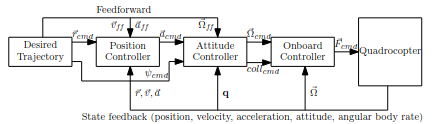
\includegraphics[scale=0.78]{../images/0001 Quadcopterregler.png}{\\Für den später verwendeten Regler wurden die Solltrajektorie zu einem Sollgeschwindigkeitsvektor vereinfacht und nur die Geschwindigkeit geregelt. Das Bild ist entnommen aus der ursprünglichen Veröffentlichung \ref{link:ETH}.}
\end{center}


\subsection{Tiefes verstärkendes Lernen}

\subsubsection{Lernproblem}
Lernen ist ein Prozess welcher darauf abzielt Zustände zu finden von welchen aus heraus der zu überblickende Aktionsraum optimaler ist als in allen vorangegangen Zuständen. 
Optimaler bedeutet der Wert des Zustandes ist maximal innerhalb der Menge aller besuchten Zustände.\\
Ein Lernproblem ist ein Problem bei welchem es im Kern darum geht Systemparameter zu finden welche zu optimalem Lernverhalten führen. 
Das Lernproblem ist eng verknüpft mit dem Teilbereich Optimierung der Elektrotechnik. 

\subsubsection{Analogien zur Regelungstechnik}
Lernende Systeme haben dasselbe Ziel wie klassische Regler sind aber in der Lage Fehler in einer Umwelt zu finden, auf die Sie nicht explizit ausgelegt wurden. Oft ist es erforderlich, dass ein Regler lernt, beispielsweise wenn sich die Reglerumwelt dynamisch ändert.\\
Tiefes verstärkendes Lernen (eng. Deep reinforcement learning) ist ein Lernparadigma das tiefe Netzwerk mit Fehlrückführungsalgorithmus und belohnungsbasierten Lernen fusioniert. Tiefe Netzwerke werden in der Regelungstechnik schon eine Weile als Regler verwendet \ref{link:Regelungstechnik2}. Eine jüngere Entwicklung ist der Einsatz des tiefen verstärkenden Lernen.
In der Regelungstechnik determinieren externe Sollwerte das Verhalten, also Werte, die aus einer Umwelt kommen, welche nicht lokal geregelt werden sollen. Im verstärkenden Lernen gibt es keine Sollwerte im Sinne der Regelungstechnik, sondern Belohnungen, welche eine Funktion der Umwelt sind, die geregelt werden soll. Will man beispielsweise die Rotationsgeschwindigkeit der Erde regeln kann man ein verstärkender Regler mit dem inversen Abstand zwischen Soll- und Istgeschwindigkeit belohnen. Auch möglich wäre die Belohnung mit der Zufriedenheit der Erdbewohner skalieren zu lassen vorausgesetzt man kann diese messen. Das Beispiel soll verdeutlichen, dass der Belohnungsbegriff einen direkteren Bezug zur Optimierung hat und mehrdeutiger ist als der Fehlerbegriff aus der klassichen Regelungstechnik.
\begin{center}
	
\includegraphics[scale=0.26]{../images/0046 Weltmodell ohne Hintergrund.png
	}{\\Modell der Erde und eindimensionalles Rotationsmodell zugleich}
\end{center}

\subsubsection{Vokabular des tiefen verstärkenden Lernens}
Tiefes verstärkendes Lernen ist ein breites Feld welches zahlreiche Lernalgorithmen umfasst. In dieser Arbeit wurde der Fokus auf modellfreie Policy-Gradient-Algorithmen, insbesondere Proximal-Policy-Optimization \ref{ppo} gelegt. Das Vokabular hat nicht den Anspruch alle Begriffe und Methoden einzuführen, sondern nur wenige die Policy-Gradient-Methoden zugrunde liegen.\\
Im verstärkenden Lernen werden Regler auch als Agenten bezeichnet. Dadurch wird unter anderem die Verbindung zur Robotik betont.\\
Der heilige Gral im verstärkenden Lernen ist das Lernen einer umweltspezifischen optimalen Strategie $\pi$ \ref{link:MaschinellesLernen}. Eine Strategie kann als Abbildung von Zuständen $s_t$ auf eine Wahrscheinlichkeitsverteilung über Aktionen $a_t$
\begin{align}
  a_t &= \pi(s_t)
\end{align}
in jedem Zeitschritt $t$ betrachtet werden \ref{link:MaschinellesLernen}. Vor dem Lernprozess ist eine Strategie zufällige initialisiert. Während dem Lernprozess ist das Ziel die Strategie so anzupassen, dass die optimale Aktion am stärksten gewichtet werden und das bei minimalem Rechenaufwand.\\
Agenten, diejenigen Entitäten deren Aktionen optimiert werden sollen, berechnen Verbesserungen ihrer Strategie im, modellfreien verstärkenden Lernen, allein basierend auf Umweltbeobachtungen und Belohnungssignalen $r_t$. Die Belohnungsfunktion
\begin{align}
  r(a_t) &= r_t
\end{align}
eine Methode der Umwelt bildet Aktionen auf Belohnungen ab. Die Summe aller zukünftigen Belohnungen ausgehend von aktuellem Zustand wird als Gewinn (eng. Gain) bezeichnet. 
\begin{align}
  G_t &= \sum_{k = 0}^{\infty}\gamma ^kr_{t+k+1}. 
\end{align}
Belohnungen kodieren, eine Anforderungen an das lernende System \ref{link:MaschinellesLernen}.
Die Zustandswertefunktion
\begin{align}
  V^\pi(s) &= E(G_t | s_t)
\end{align}
bewertet Zustände hinsichtlich des zukünftig in dem Zustand zu erwartenden Gewinn beim Handeln nach der Strategie $\pi$ \ref{link:MaschinellesLernen}.\\
Die Zustandswertefunktion kann herangezogen werden, um die Strategie zu optimieren \ref{link:MaschinellesLernen}.\\
Policy-Gradient-Methoden optimieren die Strategie auf Basis von Erfahrungssamples welche abgespeicherte Informationen aus einem Batch an Episoden sind. Eine Episode entspricht einem Prozess vom Start bis zum Ende. Für einen Agenten welcher einen Quadcopter regelt ist eine Episode beispielsweise ein Flug. Mit aktuellen Methoden des verstärkenden Lernens ist es nicht ansatzweise ausreichend marktreife Regler in einer Episode anzulernen. Weshalb der Lernprozess eines Agenten in einer Simulation passiert und oft mehrere Millionen Episoden lang läuft.

\subsubsection{Tiefe Netzwerke}
Biologisch inspirierte lernfähige Netze können konstruiert werden, indem Schichten $S$ aus Funktionen verkettet werden und die Funktionsparameter mit einem Algorithmus iterativ angepasst werden, sodass eine Verlustfunktion minimiert wird.
\begin{align}
  y &= S_1(S_2(...S_d(x)...)).
\end{align}
Sie sind in der Lage beliebige Funktionen zu approximieren \ref{link:MaschinellesLernen}. Also ihre Schätzung der oder besser Vorhersage über die Funktionswerte näher an den tatsächlichen Funktionswert zu bringen.
\subsubsection{Mehrschichtiges Perzeptronennetzwerk}
Bei einem Standardnetzwerk, dem Perzeptronennetzwerk, besteht eine Schicht $S$ aus Knoten welche die gewichteten Outputs der Knoten aus der davorliegenden Schicht summiert zu
\begin{align}
  v_j^{(S)} &= \sum_i w_{ij}^{(S)}x_i
\end{align}
und eine nichtlineare Aktivierungsfunktion $\sigma$
\begin{align}
  O_j^{(S)} &= \sigma \left (v_j^{(S)}\right )
\end{align}
auf die Summe anwendet. Die Aktivierungsfunktion ermöglicht dem Netzwerk das Lernen von wenn-dann-Beziehungen. Der Output eines Knotens wird an alle Knoten der nachfolgenden Schicht weitergeleitet.
\vspace*{0.5cm}
\begin{center}
  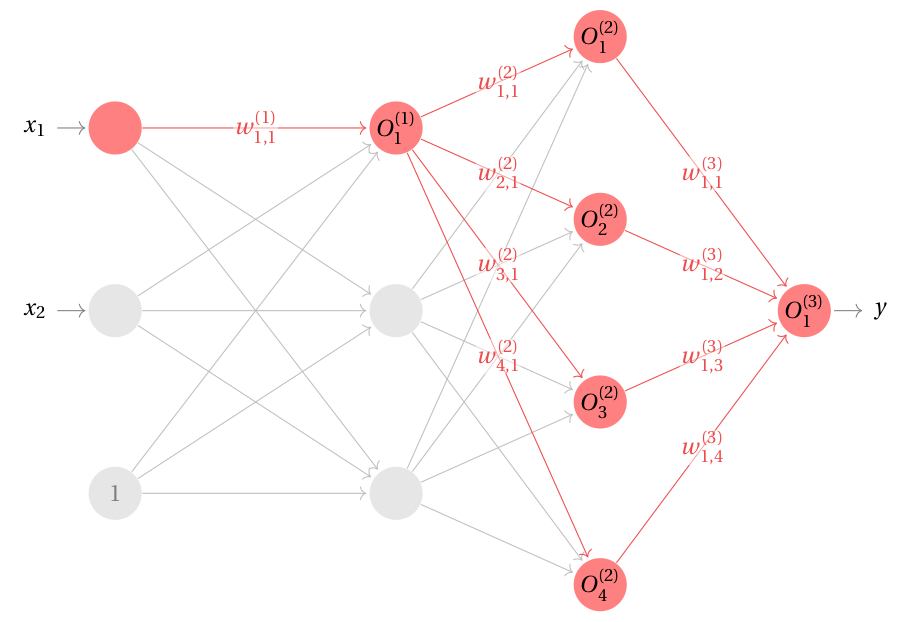
\includegraphics[
    width=0.7\textwidth, 
    keepaspectratio
  ]{../images/0032 multi-layer-perzeptron.png}{\\Ein voll verknüpftes Netzwerk in welchem alle Knoten rot sind die durch das Gewicht $w_{1,1}^{(S)}$ beeinflusst werden \ref{link:MaschinellesLernen}}
\end{center}

\subsubsection{Fehlerückführungsalgorithmus}
Die Gewichte eines Netzwerkes sollen so angepasst werden, dass der Fehler zwischen den Output des Netzwerkes $y_{Ist}$ und den Sollwerten $y_{Soll}$ minimal ist \ref{link:MaschinellesLernen}. Der Fehler $E$ wird mit einer Verlustfunktion (eng. Loss function) berechnet beispielsweise dem mittleren quadratischen Fehler
\begin{align}
  \min_{w_{ij}^{(S)}} E &= {
    \min_{w_{ij}^{(S)}}\frac{1}{2}\left (y_{\text{Soll}} - y_{Ist}\right )^2
  }.
\end{align}
Das entwickelte Optimierungsproblem, für die Gewichte $w_{ij}^{(S)}$, wird iterativ mit dem Gradientenabstiegsverfahren 
\begin{align}
  w_{ij,t+1}^{(S)} &= {
    w_{ij, t}^{(S)} - \mu \frac{\partial E}{\partial w_{ij, t}^{(S)}}
  }
\end{align}
gelöst bei einer Lernrate $\mu $ \ref{link:MaschinellesLernen}.\\
Die partielle Ableitung der Verluste als Funktion der Gewichte kann berechnet werden durch die Anwendung der Kettenregel
\begin{align}
  \frac{\partial E}{\partial w_{ij}^{(S)}} &= {
    \sum_j \left (y_{\text{Soll}} - y_{\text{Ist}}\right )\frac{\partial y}{\partial w_{ij}^{(S)}}
  }.
\end{align}
Der Output des Netzwerks $y_{Ist}$ entspricht dem Output der letzten Schicht des Netzwerks
\begin{align}
  \frac{\partial E}{\partial w_{ij}^{(S)}} &= \sum_j \left (y_{\text{Soll}} - y_{\text{Ist}}\right )\frac{\partial \sigma \left (v_j^{(S)}\right )}{\partial w_{ij}^{(S)}}.
\end{align}
Die Kettenregel wird erneut verwendet um die partielle Ableitung der Aktivierungsfunktion nach den Gewichten zu berechnen
\begin{align}
  \frac{\partial E}{\partial w_{ij}^{(S)}} &= \sum_j \left (y_{\text{Soll},j} - y_{\text{Ist}}\right )\sigma'\left (v_j^{(S)}\right )\frac{\partial v_j^{(S)}}{\partial w_{ij}^{(S)}}.
\end{align}
Die Inputgewichte werden proportional zum Fehler, der Aktivierung und dem Output des Netzwerks
\begin{align}
  \frac{\partial E}{\partial w_{ij}^{(S)}} &= \sum_j \left (y_{\text{Soll},j} - y_{Ist, j}\right )\sigma'\left (v_j^{(S)}\right )O_j
\end{align}
aktualisiert \ref{link:MaschinellesLernen}.

\subsection{\label{ppo}Proximal-Policy-Optimization}
Proximal-Policy-Optimization ist ein Policy-Gradient-Algorithmus aus dem Bereich des tiefen verstärkenden Lernens \ref{link:PPOSpinningUp}.\\
Kernelement von Proximal-Policy-Optimization sind zwei tiefe Netzwerke welche im Sinne einer Actor-Critic-Architektur zusammen fungieren. Die Idee dabei ist, dass Aktionen eines Strategienetzwerks kontinuierlich bewertet beziehungsweise kritisiert werden durch ein Netzwerk welches die Zustandswertefunktion approximieren. Das Strategienetzwerk nimmt die Rolle des Actors ein und das Zustandswertenetzwerk die des Critics.\\
Proximal-Policy-Optimization lernt nicht in jedem \textit{step} die Strategie, sondern nach einer oder mehreren Episoden \ref{link:PPOSpinningUp}. Diese Form des agieren auf der Umwelt mit der probabilistischen Strategie wird Rollout genannt. Um alle Aktionswahrscheinlichkeiten, Aktionen, Beobachtungen und Belohnungen, seit der letzten Lernphase, für die Optimierung einzubeziehen werden diese in Batches abgespeichert. Es gilt des weitern Verlustfunktionen zu berechnen um die Strategie- und Zustandswertenetzwerke zu optimieren. Aufseiten des Critics erfolgt dies auf Basis der gespeicherten Belohnungen, den sogenannten Unterwegsbelohnungen und der Vorhersage des aktuellen Zustandswertenetzwerks. Das Fehlermaß wird für die Verlustfunktion ist der Euklidische Abstand zwischen den tatsächlich erfahrenen Belohnungen $R$ und der aktuellen Annahme für $V^{\pi}$.\\
Für die Optimierung des Actors wird die Zustandswertefunktion als Kritik herangezogen. Durch Subtraktion der Zustandswerte einer Episode von den gesammelten Unterwegsbelohnungen wird auf Vorteile (eng. Advantages) A geschlossen. Diese quantifizieren die Güte der aktuellen Aktion im Vergleich zu allen möglichen Aktionen eines Zustandes.
Die Auftrittswahrscheinlichkeit der vom Actor gewählten Aktion zur letzten wird ratio genannt und bemisst die Divergenz zwischen neuer und alter Strategie. Das logarithmieren der Wahrscheinlichkeiten hilft beim Gradientenabstieg \ref{link:LogPPO}.
Eine zentrale Innovation von Proximal-Policy-Optimization gegenüber Vorgängern ist das der ratio auf den Wertebereich 0.8 und 1.2 eingekürzt wird. Durch diese Maßnahme wird sichergestellt, dass Aktionen nur gering voneinander abweichen. Der Lernprozess wird einheitlicher, konservativer und damit stabiler \ref{link:PPOSpinningUp}.
Durch die Multiplikation von Vorteilen A und ratio, siehe Bild, werden Hilfsfunktionen (eng. surrogate function) $S_1$ und $S_2$ berechnet. Durch Minimierung und Mittelwertbildung wird auf die Verluste für das Strategienetzwerk geschlossen.
\begin{center}
    \begin{tikzpicture}[font=\sffamily,every label/.append
    style={font=\small\sffamily,align=center}]

	\node[doc] at (1, 0) (Regler) {Rollout};

	\node[
		cylinder, 
		cylinder uses custom fill, 
		cylinder end fill=orange!25,
		cylinder body fill=orange!50,
		shape border rotate=90,
		text=white,
		aspect=0.4,
		minimum width=1cm,
		minimum height=1.4cm] at (4, -2) (BatchBelohnungen){Unterwegsbelohnung $R$};

	\node[cylinder, cylinder uses custom fill, cylinder end fill=violet!25,
	cylinder body fill=violet!25,shape border rotate=90,text=white,
	aspect=0.4,minimum width=1cm,minimum height=1.4cm] at (4, 0) (BatchLog){Log $log(p_{a,t-1})$};

	\node[cylinder, cylinder uses custom fill, cylinder end fill=red!25,
	cylinder body fill=red!50,shape border rotate=90,text=white,
	aspect=0.4,minimum width=1cm,minimum height=1.4cm] at (4, 2) (BatchAktionen){Aktionen $p_{a}$};

	\node[cylinder, cylinder uses custom fill, cylinder end fill=blue!25,
	cylinder body fill=blue!50,shape border rotate=90,text=white,
	aspect=0.4,minimum width=1cm,minimum height=1.4cm] at (4, 4) (BatchBeobachtungen){Beobachtungen $o$};

	\node[doc] at (7, 2) (Critic) {Actor};

	\node[doc] at (8, 4) (Evaluate) {Critic};

	\node[doc] at (7, 0) (Ratios) {$e^{x-y}$};

	\node[doc] at (7, -4) (Clamp) {Clip($0.8, 1.2$)};

	\node[circle, draw] (Advantage) at (8, -2) {-};

	\node[circle, draw] (Surr1) at (9, -2) {$\cdot$};

	\node[circle, draw] (Surr2) at (9, -3) {$\cdot$};

	\node[doc] at (12.25, -5) (MSE) {$\sqrt{R^2 - {V^{\pi}}^2}$};

	\node[doc] at (15.5, -2) (Backprop1) {Actor update\\$w_{ij} - \mu \frac{\partial L_{Actor}}{\partial w_{ij}^{(l)}}$};

	\node[doc] at (15.5, -5) (Backprop2) {Critic update\\$w_{ij} - \mu \frac{\partial L_{Critic}}{\partial w_{ij}^{(l)}}$};

	\node[doc] at (11, -2) (Mean) {$\overline{\min{S_1, S_2}}$};

	\draw[-latex] (Regler) |- (BatchBelohnungen);

	\draw[-latex] (Regler) |- (BatchAktionen);

	\draw[-latex] (Regler) |- (BatchBeobachtungen);

	\draw[-latex] (Regler) -- (BatchLog);

	\draw[-latex] (BatchBeobachtungen) -- (Evaluate);

	\draw[-latex] (BatchAktionen) -- (Critic);

	\draw[-latex] (BatchLog) -- (Ratios);

	\draw[-latex] (Evaluate) -- (Advantage) node[midway, above, font=\small\sffamily]{};

	\draw[-latex] (BatchBelohnungen) -- (Advantage);

	\draw[-latex] (Critic) -- (Ratios) node[midway, left, font=\small\sffamily]{$log(a)$};

	\draw[-latex] (Advantage) -- (Surr1) node[midway, below, font=\small\sffamily]{$A$};

	\draw[-latex] (Ratios) -| (Surr1) node[midway, right, font=\small\sffamily]{$ratio$};

	\draw[-latex] (Ratios) -- (Clamp);

	\draw[-latex] (Clamp) -| (Surr2) node[midway, right, font=\small\sffamily]{$clipped\ ratio$};

	\draw[-latex] (Advantage) |- (Surr2) node[midway, left, font=\small\sffamily]{$A$};

	\draw[-latex] (Surr1) -- (Mean) node[midway, below, font=\small\sffamily]{$S_1$};

	\draw[-latex] (Surr2) -| (Mean) node[midway, below, font=\small\sffamily]{$S_2$};

	\draw[-latex] (Mean) -- (Backprop1) node[midway, below, font=\small\sffamily]{$L_{Actor}$};

	\draw[-latex] (Evaluate) -| (MSE) node[midway, above, font=\small\sffamily]{$V^{\pi}$};

	\draw[-latex] (BatchBelohnungen) |- (MSE) node[midway, above, font=\small\sffamily]{};

	\draw[-latex] (MSE) -- (Backprop2) node[midway, above, font=\small\sffamily]{};

	\draw[-latex] (BatchBeobachtungen) -| (Critic) node[midway, above, font=\small\sffamily]{};
	\end{tikzpicture}
\end{center}
Diese Einführung zu Proximal-Policy-Optimization hat nicht den Anspruch eine vollumfängliche Implementierung zu ermöglichen. Vielmehr sollen die Grundlegenden Gedanken angesprochen werden. Für mehr Details empfielt es sich \ref{link:PPOBeginner} zu studieren.

\subsection{Stable-Baselines3}
Stable-Baselines3 implementiert Algorithmen und abstrahiert diese für das Verstärkende Lernen in der Programmiersprache Python. \label{paralleleUmwelten}Zudem, umfasst die Bibliothek weiter Funktionen, so lassen sich Modelle parallel in mehreren Umwelten trainieren, wodurch die Lerngeschwindigkeit, insbesondere auf Grafikkarten, maximiert werden kann. Ein weiterer Vorteil von Stable-Baselines3 ist, dass verschiedene Optimierungen vorgenommen worden sind, um die Lerngeschwindigkeit von Algorithmen wie Proximal-Policy-Optimization zu steigern. In \textit{stablebaselines3.py} wurden eine Reihe der angesprochenen Features implementiert. Die Klasse Umwelt implementiert die Umweltdynamik, ein Grundgerüst dieser wird in \ref{gymnasium} dargestellt.\\
Die Implementierung eines Algorithmuses reduziert sich mit Stable-Baselines3 auf das Importieren der Bibliothek, hier PPO und die Definition mitsamt Hyperparameter Übergabe. Zunächst wird der Netzwerktyp übergeben, MlpPolicy steht dabei für tiefes Perzeptronennetzwerk (eng. Multi Layer Perceptron). Der zweite Parameter im Beispiel ist die Umwelt welche vorher mit der Funktion \textit{make\_vec\_env} parallelisiert wurde. Das Lernverhalten des Modells wird mit Tensorboard aufgezeichnet in den spezifizierten Ordner. Die Daten können unter Linux durch das Ausführen des Befehls \textit{tensorboard --logdir=tensorboard} im Browser dargestellt werden. Weitere Details zu Tensorboard im Abschnitt \ref{tensorboard}. Das übergebene Dictionary enthälte Informationen zur Netzwerktopologie der Stragie- und Zustandsnetzwerke. Der nächste Parameter ist ein wichtiger Hyperparameter, die Lernrate des Gradientenabstiegsverfahren. Zuletzt wird die Batchgröße spezifiziert.\\
Durch aufrufen der Methode \textit{learn} beginnt der Lernprozess. Speziell an der dargestellten Implementierung ist, dass mit einem Callback das beste Modell periodisch zwischengespeichert wird. 
\begin{center}
    \begin{tikzpicture}[font=\sffamily,every label/.append
    style={font=\small\sffamily,align=center}]
    
    \node[doc, fill=white] (Quadcontroller) {stablebaselines3.py\\  \begin{lstlisting}[language=Python, basicstyle=\fontsize{8}{10}\selectfont]
import torch
from umwelt import Umwelt
from stable_baselines3 import PPO
from stable_baselines3.common.env_util import make_vec_env
from stable_baselines3.common.callbacks import CallbackList

class Agent():
    def __init__(self):
        super(Agent, self).__init__()
	self.ordnername = f"./Modelle/{config.Ordnername}/model"
        self.train()

    def train(self):
        # Vektorisiertes Environment
        env = Umwelt()
        envs = make_vec_env(Umwelt, seed, n_envs)
        # Architektur des Neuronalen Netzwerks
        policy_kwargs = dict(
            activation_fn = torch.nn.Tanh,
            net_arch = dict(pi = config.pi, vf = config.vf)
        )
        # Proximal policy optimization Initialisierung
        self.model = PPO(
            "MlpPolicy",
            self.envs,
            tensorboard_log = self.ordnername,
            policy_kwargs = policy_kwargs,
            learning_rate = config.lernrate,
            batch_size = config.batchmenge,
        )
        # Starten des Lernprozesses
        self.model.learn(
            config.episoden,
            callback = CallbackList([
                HyperparameterParamCallback(),
                save_best_model_callback
            ])
        )
	# Trainiertes Modell abspeichern
	self.model.save(self.ordnername)

if __name__ == "__main__":
    agent = Agent()
        \end{lstlisting}
    };
    \end{tikzpicture}
\end{center}

\subsection{\label{gymnasium}Famara Gymnasium}
In Kombination mit Stable-Baselines3 kann Famara Gymnasium eingesetzt werden zur Definition von einer Klasse mit standardisierten Methoden in welcher Umweltlogik implementiert werden kann. Der Anwender muss die Methoden   \textit{reset} und \textit{step} definitonskonform implementieren, alles andere übernimmt die Bibliothek.\\
Zunächst wird die Umwelt initialisiert. Daraufhin beginnt eine Episode welche andauert bis \textit{terminated} oder \textit{truncated} Wahr wird und ist gekennzeichnet durch das periodisch ausführen von \textit{step}. Wird die Episode abgeschlossen empfielt sich die Verwendung von \textit{terminated} wird Sie abgeborchen sollte \textit{truncated} Wahr gesetzt werden. Optional kann in jedem Schritt die Umwelt gerendert werden mit der Methode \textit{render}.\\
Stable-Baselines3 hat eine Reihe an Funktionen welche die Konfiguration vor dem Training und die Überwachung des Trainingsprozesses ermöglichen. Darunter eine beispielsweise eine Fortschrittsanzeige welche die aktuelle Episode visualisiert.
\begin{center}
    \begin{tikzpicture}[font=\sffamily,every label/.append
    style={font=\small\sffamily,align=center}]
    
    \node[doc, fill=white] (Quadcontroller) {gymnasiumenv.py\\  \begin{lstlisting}[language=Python, basicstyle=\fontsize{8}{10}\selectfont]
import gymnasium as gym
import numpy as np
from gymnasium import spaces

class Umwelt(gym.Env):
    def __init__(self):
        super(Umwelt, self).__init__()
		
        # Spezifikation des Aktionsraumes
        self.action_space = spaces.Box(
		low = -1, high = 1, shape = (4,), dtype = numpy.float32
	)
        # Spezifikation des Beobachtungsraumes 
        self.observation_space = spaces.Box(
            low = -3, high = 3, shape = (9,), dtype = numpy.float32
        )

    def reset(self, seed=None, options=None):
        # Episode zuruecksetzen
        return self.state, info

    def step(self, action):
	# Schritt auf Umwelt ausfueren
        ...
        return self.state, reward, terminated, truncated, info

    def render(self):
		...
		\end{lstlisting}
    };
    \end{tikzpicture}
\end{center}

\subsection{\label{tensorboard}Tensorboard}
Tensorboard ist ein Set an Programmen zur Visualisierung von PyTorch oder TensorFlow Lernprozessen \ref{link:DeepReinforcementLearning}. PyTorch und TensorFlow sind zwei der meistgenutzten Python Bibliotheken im Gebiet des Tiefen Verstärkenden Lernen. Verschiedene Metriken und Parameter können beim Training gespeichert werden und anschließend im Browser über einen lokalen Port visualisiert werden. Besonders wichtig sind die Episodenlänge und die Episodenbelohnung. Die Länge einer Episode entspricht der Anzahl an Schritten eines Agenten. 
\begin{center}
	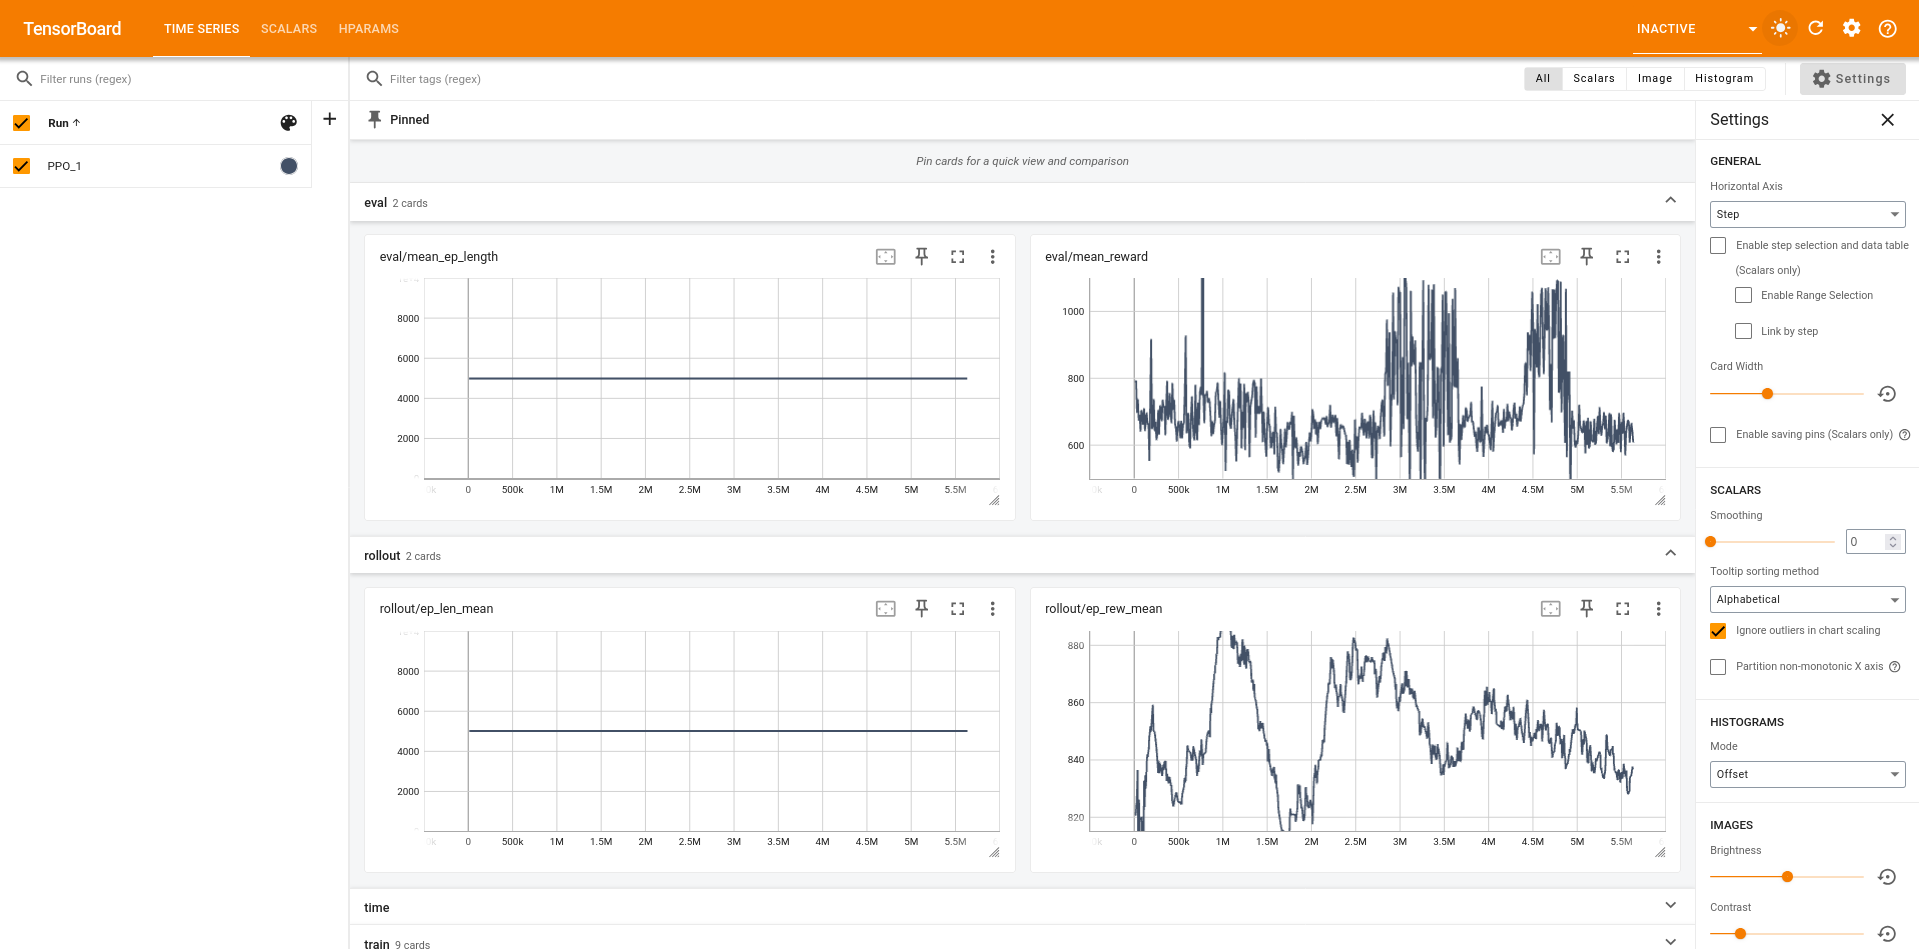
\includegraphics[width=0.98\textwidth, keepaspectratio]{../images/0058 Tensorboard.png}{\\Tensorboard welches ein Training mit PPO zeigt bei dem die mittlere Episodenanzahl konstant ist und die Belohnung im Rollout und in der Evaluation nicht wie gewünscht kontinuirlich steigt.}
\end{center}

\subsection{Zustandsobservation mit einer Inertialen Messeinheit}
Eine Inertiale Messeinheit (eng. Inertial Measuring Unit (IMU)) ist ein System welches in der Regel Beschleunigungssensoren und Drehratensensoren, manchmal auch Magnetfeldsensoren zusammenfasst. Die Bündelung der Sensoren hat sich etabliert da Sensorrohdaten aus den genannten Sensoren häufig fusioniert werden, zur Schätzung von Drehlage und linearer, also um den Gravitationsvektor gefilterte, Beschleunigung. Sensortechnologien wie Laufzeit-, Feldstärke- und Winkelmessung oder Inertialsensorik besitzen prinzipiell komplementäre Eigenschaften in Bezug auf Reichweite, Präzision oder Abtastgeschwindigkeit \ref{link:Sensorfusion}.
Komplementär- und Kalman-Filter sind Beispiele für Sensorfusionsalgorithmen. Auch Methoden des tiefen Lernens eignen sich zur Sensordatenfusion \ref{link:DeepLearningStateEstimation}.\\
Mikrocontrollerhersteller veröffentlichen neben Sensorhardware in der Regel auch Beispielprogramme welche das Auslesen und die Sensordatenfusion demonstrieren.\\
STMicroelectronics bietet die Erweiterung X-CUBE-MEMS1 an welche mit der Bibliothek MotionFX genutzt werden wird zur Sensorfusion \ref{X-CUBE-MEMS1}.

\subsection{Pulsweitenmodulation und Motoransteuerung}
Pulsweitenmodulation (PWM) ist ein Verfahren zur Signalmodulation. PWM-Signale werden unter anderen verwendet zur Ansteuerung von BLDC-Motoren.\\
Bausteine einer mikrocontrollerbasierten Pulsweitenmodulation sind ein Timer und eine Capture/Compare Einheit welche eine Ganzzahl (eng. integer) $n$ hochzählt und mit einem Wert im Capture-Compare-Register (CCR) vergleicht (eng. compare). Ist der Wert des Zählers größer als der Wert im Register wird die Spannung am Output auf Ground gezogen. Zu Beginn beziehungsweise Ende von jeder Periode, dessen Länge durch die Frequenz des Timers bestimmt ist, wird die Spannung beispielsweise auf 3.3V gesetzt. 
\begin{align}
	u(t) &= \left\{\begin{array}{ll} 3.3V, & n < CCR\ \text{mit}\ n\in N\ \text{und}\ n\in [0, CCR]\\
		0, &\text{sonst}\end{array}\right. .
\end{align}
Abhängig vom Pegel stellt sich ein Signal ein welches einen Duty-Cycle $d$ hat der dem Quotient aus Pegel und dem höchsten Wert des Capture-Compare-Registers entspricht. 
\begin{align}
	D &= \frac{n}{\max{(CCR)}}
\end{align}
Der artihmetische Mittelwert des PWM-Signals $u(t)$ ist dann proportional zum Duty-Cycle.
\begin{align}
	\bar{u} &= 3.3V\cdot d
\end{align}
BLDC-Motoren werden wegen ihres Aufbaus zur Klasse der Gleichstrommotoren gezählt\\ benötigen aber jeweils um 120° versetzte periodische, stückweise gleichförmige, Signale an den drei Anschlüssen. Diese Signale können mithilfe von PWM-Signalen aus einem Mikrocontroller generiert werden wobei der Duty-Cycle die Leistungsteuerung und damit die Drehmomentregelung des Motors ermöglicht. Da die Leistung von Mikrocontrollerpins auf 3.3V begrenzt ist, werden in der Praxis noch Leistungstransistoren wie MOSFETs oder IGBTs, sowie eine externe Spannungsquelle zwischengeschaltet. Sowohl die Funktion der Signalgeneration für den BLDC-Motor aus auch, die der Leistungselektronik sind in BLDC-Motortreibern integriert, durch welche der Entwicklungsprozess von Anwendungen mit BLDC-Motoren deutlich beschleunigt wird. Der Entwicklungsaufwand reduziert sich auf die Verschaltung des Treibers und die Generation eines PWM-Signal dessen Duty-Cycle das Motordrehmoment steuert.

\subsection{Flask und ThreeJS}
Flask ist eine Python Bibliothek welche das Programmieren von Webanwendungen vereinfacht \ref{link:Flask}. In Kombination mit der Javaskript Bibliothek ThreeJS lassen sich vergleichsweise schnell 3D-Anwendungen für den Browser entwickeln. Im Netz zugänglich ist neben der ThreeJS Dokumentation eine umfangreiche Zusammenstellung von Beispielen.
\begin{center}
	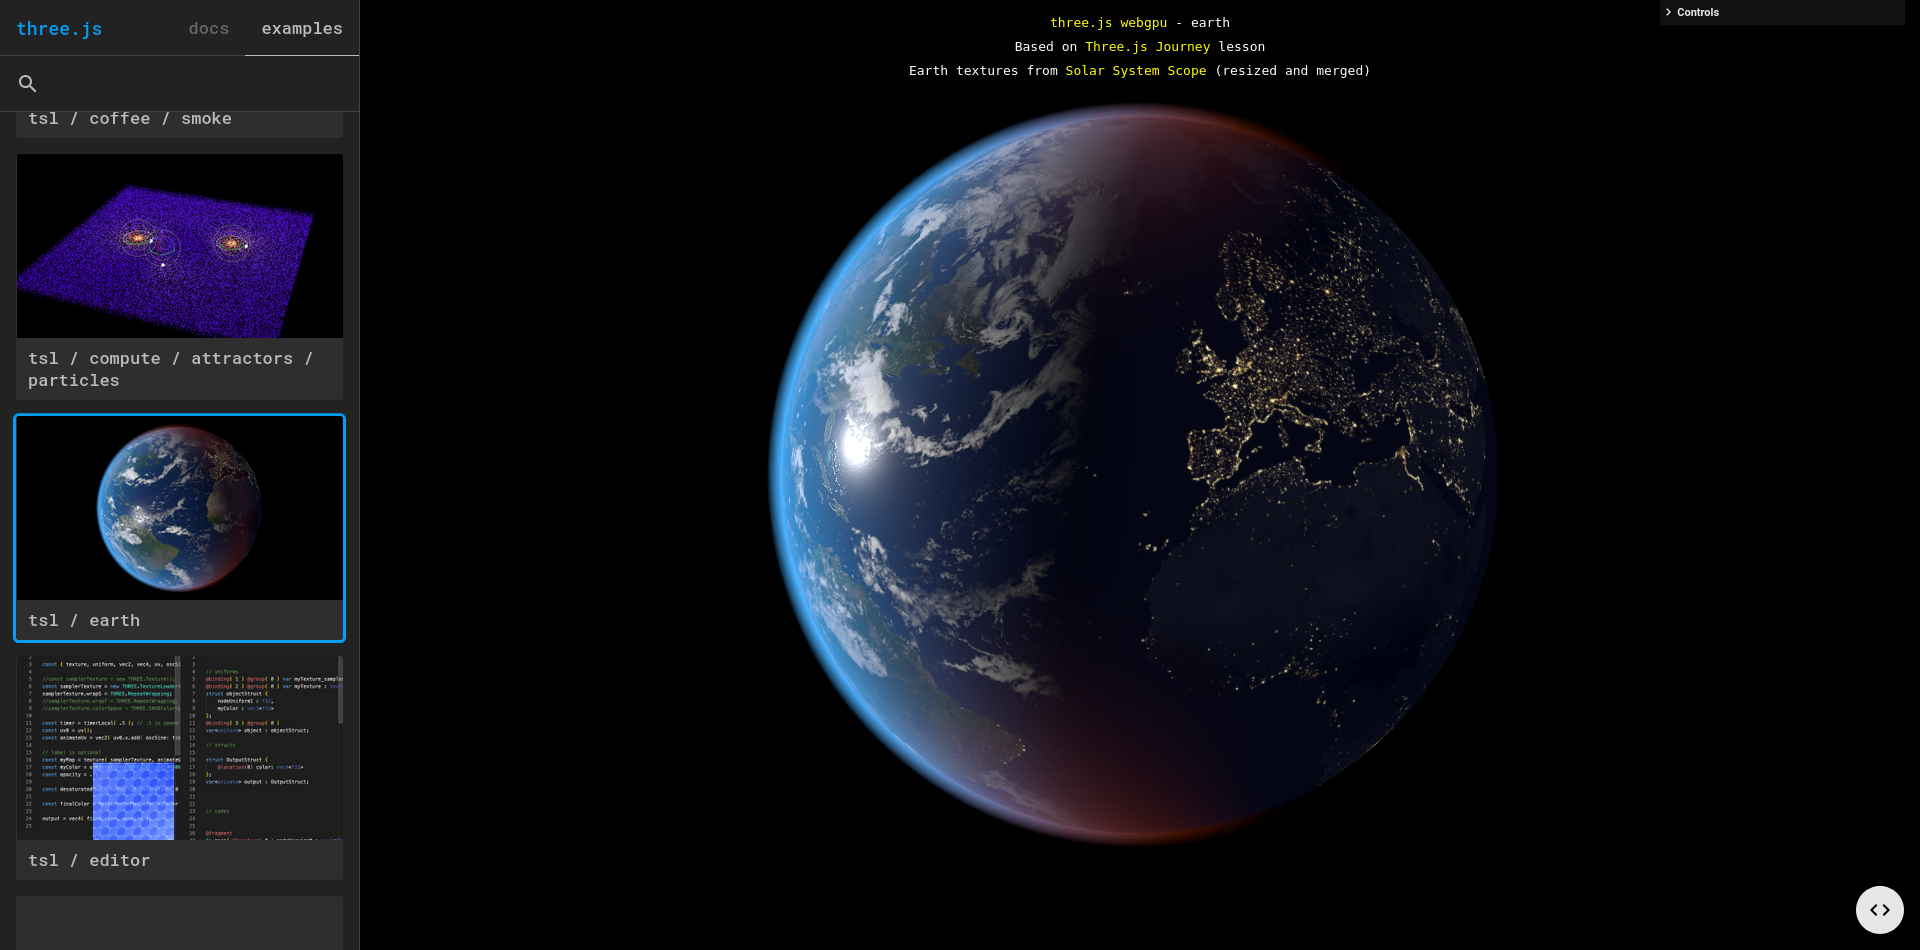
\includegraphics[width=0.9\textwidth, keepaspectratio]{../images/0062 ThreeJS Beispielselektor.png}{\\ThreeJS Beispielselektor mit Beispiel tsl/earth gewählt \ref{bild:3}}
\end{center}